% 04-mpu.tex

\section{Memory Protection Unit (MPU) Implementation}

\begin{frame}{Overview}
    \begin{itemize}
        \item The MPU enhances security by restricting memory access based on region configurations.
        \item The ARM Cortex-M7 processor supports up to 16 MPU regions.
        \item FreeRTOS provides built-in MPU support for ARM Cortex-M4, which can be theoretically adapted for Cortex-M7.
        \begin{itemize}
            \item \textbf{Errata 837070}: Requires workarounds for Cortex-M7 r0p0 and r0p1 revisions. 
        \end{itemize}
    \end{itemize}
\end{frame}

\begin{frame}{MPU Configuration}
    \begin{columns}
        \column{0.6\textwidth}
        \begin{itemize}
            \item Each MPU region is configured with:
            \begin{itemize}
                \item Base address
                \item Region size
                \item Access permissions (privileged/unprivileged, read/write/execute)
            \end{itemize}
            \item Enables separation of kernel and user-mode tasks.
        \end{itemize}
        \column{0.4\textwidth}
        \centering
        
\includegraphics[width=0.7\linewidth]{../images/mpu_meme.png}
    \end{columns}
\end{frame}

\begin{frame}{Theoretical Steps for Implementation}
    \begin{itemize}
        \item \textbf{Define MPU Region Count in \texttt{FreeRTOSConfig.h}}:
            \begin{itemize}
                \item Set \texttt{configENABLE\_MPU} to 1.
                \item Set \texttt{configTOTAL\_MPU\_REGIONS} to 16.
                \item Set \texttt{configENABLE\_ERRATA\_837070\_WORKAROUD} to 1.
            \end{itemize}
        \item \textbf{Enable Errata Workaround}: Apply fix for Cortex-M7 r0p0 and r0p1 by modifying \texttt{port.c}.
        \item \textbf{Integrate FreeRTOS Changes}: Adapt \texttt{ARM\_CM4\_MPU/port.c} to support Cortex-M7.
    \end{itemize}
\end{frame}

\begin{frame}{MPU in QEMU}
    \begin{itemize}
        \item \textbf{Device Tree (qtree)}
        \begin{itemize}
            \item Used \texttt{qtree} to inspect the device tree of the board.
            \item Found two MPU regions, each containing 8 blocks.
        \end{itemize}
        \item \textbf{Script Execution}
        \begin{itemize}
            \item Ran a script to determine how many MPU regions exist in a block.
        \end{itemize}
        \begin{figure}[h]
            \centering
            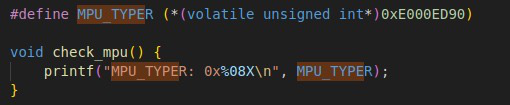
\includegraphics[width=0.75\textwidth]{images/mpu_qemu_1.png}
            \caption{MPU Region Detection Script}
        \end{figure}
    \end{itemize}
\end{frame}

\begin{frame}{MPU in QEMU}
    \begin{itemize}
        \item \textbf{Result Analysis}
        \begin{itemize}
            \item The script returned \texttt{0x00000800}.
            \item \textbf{Bit 0 (MPU Present Bit)} = 0 
            \begin{itemize}
                \item Some Cortex-M chips use this bit to indicate MPU presence.
                \item For Cortex-M7 (S32K3 series), this bit is always 0. 
            \end{itemize}
            \item \textbf{Bits 15:8 (DREGION)} = 8  
            \begin{itemize}
                \item MPU supports 8 regions.
            \end{itemize}
        \end{itemize}
        \begin{figure}[h]
            \centering
            
\includegraphics[width=0.75\textwidth]{images/mpu_qemu_2.png}
            \caption{MPU Detection Result}
        \end{figure}
    \end{itemize}
\end{frame}